\documentclass[twoside,11pt,openright,a4paper]{report}

\usepackage{cstitle}
\usepackage[utf8]{inputenc}
\usepackage[american]{babel}
\usepackage{latexsym}
\usepackage{amssymb}
\usepackage{amsmath}
\usepackage{epsfig}
\usepackage[T1]{fontenc}
\usepackage{lmodern}
\usepackage{color}
\usepackage{datetime}
\usepackage{epstopdf}
\usepackage{hyperref}

\usepackage{csquotes}
\usepackage{listings}
\usepackage[backend=biber]{biblatex}
\usepackage{cite}

\usepackage{minted}
\usepackage{float}
\floatstyle{boxed}
\restylefloat{figure}

\addbibresource{refs.bib}

\hypersetup{
    pdfborder = {0 0 0}
}
\newcommand{\remark}[1]{{ \bf [ \footnotesize #1 ]}}
%\newcommand{\remark}[1]{}
\newcommand{\orangutan}{Orangutan}
\newcommand{\bibtex}{Bib{\TeX}}
\newcommand{\chapref}[1]{(Section~\ref{#1})}
\newcommand{\rfquote}[2]{
\begin{flushright}
\emph{#1}\\
-- #2
\end{flushright}}

\newcommand{\figref}[1]{Figure~\ref{#1}}
\newcommand{\ie}{i.e.}
\newcommand{\eg}{e.g.}
\newcommand{\newdef}[1]{`#1'}
\newcommand{\file}[1]{.#1 file}

\graphicspath{ {graphics/} {./} }
% see http://imf.au.dk/system/latex/bog/

\begin{document}
\pagestyle{empty}
\pagenumbering{Alph}
\begin{titlepage}
\author{Rohde Fischer - 20052356}
\csAdvisor{Olivier Danvy}
\title{An automated approach\\to organizing {\bibtex} files}
\maketitle

\end{titlepage}

%%%%%%%%%%%%%%%%%%%%%%%%%%%%%%%%%%%%%%%%%%%%%%%%%%%%%%%%%%%%%%%%%%%%%%%

\pagestyle{plain}
\setcounter{page}{1}


\chapter*{Abstract}
\addcontentsline{toc}{chapter}{Abstract}

We successively describe the bibliographic software tool {\bibtex}
(both how to use it in principle and how it is used in practice), list
a range of practical issues {\bibtex} users encounter, propose an
approach to hand\-ling these issues, and review how they are tackled
in related work.  We then present an analysis of {\bibtex} files that
detects these issues and we describe how to solve them by organizing
{\bibtex} files using the results of the analysis.  We implemented a
proof of concept, {\orangutan}, that analyzes existing {\bibtex} files
and emits diagnostics and suggestions.


\chapter*{Resumé}
\addcontentsline{toc}{chapter}{Resumé}

%\chapter*{Acknowledgements}
%\addcontentsline{toc}{chapter}{Acknowledgments}
%
%\vspace{2ex}
%\begin{flushright}
%  \emph{Olivier Danvy,}\\
%  \emph{Aarhus, \today.}
%\end{flushright}

\tableofcontents
\newpage

\pagenumbering{arabic}
\setcounter{secnumdepth}{2}

%%%%%%%%%%%%%%%%%%%%%%%%%%%%%%%%%%%%%%%%%%%%%%%%%%%%%%%%%%%%%%%%%%%%%%%

\chapter{Introduction}
\label{ch:intro}
This dissertation documents a method for automated detection of
lexical and inconsistency concerns in {\bibtex} references.

\chapter{{\bibtex}}
\label{ch:about}
\section{Introduction}
The goal of this chapter is to introduce {\bibtex}: the course of
events leading to {\bibtex} \chapref{sec:why_bibtex_came_to_be}, what
{\bibtex} is \chapref{sec:principles_of_bibtex}, how {\bibtex} is used
in principle \chapref{sec:practice_of_bibtex}, and how {\bibtex} is
used in practice \chapref{sec:how_bibtex_is_used_today}.


\section{Why {\bibtex} came to be}
\label{sec:why_bibtex_came_to_be}

The advent of {\TeX} has been a game changer for scientific writing,
witness the number of articles written in {\TeX} (or derivatives such
as {\LaTeX}).  For instance, on arXiv.org, nearly all articles are
formatted with \LaTeX.  Apart from being grateful to Donald Knuth for
providing such a robust system for scientific articles, writers can
also be thankful that {\TeX} has given the basis for Oren Patashnik
and Leslie Lamport to create {\bibtex} for managing scientific
bibliographies.

Before the wake of {\bibtex}, bibliographic references were managed
entirely by hand and required a lot of labor.  For instance, nearly
half of Mary-Claire van Leunen's book, \textit{A Handbook for
  Scholars}~\cite{leunen1992_handbook}, is dedicated to citing,
managing, and writing references, \ie, 150 pages out of 335 pages
(excluding the index).  Likewise, a significant fraction of Umberto
Eco's book, \textit{How to Write a Thesis}~\cite{eco1985_thesis}, is
also dedicated to managing and citing references and to ensuring a
proper bibliography.  All this manual labor has almost been made
obsolete by {\bibtex}.

Even more, {\bibtex} entries are now readily available online, and so
the practical problem of bibliographic references is now solved, in
principle.

\section{What is {\bibtex}}
\label{sec:principles_of_bibtex}

In the same spirit as {\LaTeX}, {\bibtex} is a simple software tool
for managing bibliographic references in scientific writing, using an
ASCII file to specify theses references.  Inside this ASCII file, the
components of each reference are specified, such as the author, title,
year and what kind of medium (\eg, a book or article) was used.  This
file will be referred to as \newdef{the {\bibtex} file} or
\newdef{\file{bib}}

Depending on the forum, there are differences in: how references
should be cited, be written, and the order in which they should be listed.
Each publisher has a mandatory setup.  The specific set of rules a
publisher has is referred to as a \newdef{bibliography style} or
\newdef{citing style}.

When processing a document, {\bibtex} cites according to the selected
bibliography style, ensures the formatting and the order in the
reference list, and ensures that only relevant entries are included.
The references are labeled consistently in the document according to
the citing style, the labels are used when a reference is cited and
these labels allows the reader to quickly find the reference in the
bibliography, as illustrated in \figref{fig:bibtex_example_alpha}.

Today, {\bibtex} has also enabled huge online resources with
references, automated extraction tools, sharing of references and easy
version control.  The {\bibtex} format is originally designed for use
with {\LaTeX}, but it has plugins for other formats as
well~\cite{bibtex_resource}.

\begin{figure}
  \centering
  
\includegraphics[width=0.8\textwidth]{bibtex-styles-ex-acm}
  \caption{{\bibtex} output using ACM citing style which uses numbers to
    index entries.  Source: ShareLaTeX~\cite{sharelatex2016_styles}}
\label{fig:bibtex_example_acm}
\end{figure}

\section{How {\bibtex} is used in principle}
\label{sec:practice_of_bibtex}

\subsection{Macro-use}

A {\bibtex} file consists of entries each corresponding to a
bibliographic reference, such as an article or a book.  Each entry in
turn contains meta information about the reference, through tags that
specify the kind of meta information such as the author or title.
Also, quite commonly, a file will contain a lot of shortenings for
text fragments that are reused.

To select the desired style the command
${\backslash}bibliographystyle$ is used, for example
${\backslash}bibliographystyle\{alpha\}$.  The style in turn controls
the formatting and how the references are labeled, as can be seen on
\figref{fig:bibtex_example_acm} and \figref{fig:bibtex_example_alpha}
where the labels are different, the abbreviation of author names are
different and some of the visual formatting is different.

To build a {\LaTeX}-document with {\bibtex} references in it, one
first runs the $latex$ command (or one of the derivatives) to produce
(among other things) an \file{aux}.  The \file{aux} contains auxiliary
information from the {\LaTeX}-compiler.  Then run the $bibtex$ command
which uses the \file{aux} to find the entries in use and to give them
labels according to the reference style.  The output from {\bibtex} is
a \file{bbl} with the formatted references, which is then used by
subsequent runs by {\LaTeX}, so the document will have labels at the
appropriate places and an bibliography in accordance with the labels.


\subsection{Micro-use}

Inside a {\bibtex} file, the format itself is fairly simple. At the
main level, we have $@STRING$, $@PREAMBLE$, $@COMMENT$ and $entries$.
$@STRING$ is for shortenings that can be used later in the {\bibtex}
file, $@PREAMBLE$ is for defining how to format the text and
$@COMMENT$ is for comments and $entries$.  The $entries$ correspond to
the different medium types, such as $@ARTICLE$, $@BOOK$ and
$@PROCEEDINGS$, which in turn contain the relevant tags for the given
entry.  Each entry consist of an identifying key and a set of tags.
The identifying key will be called \newdef{entry key} to avoid
ambiguity with the tag $key$.  For each entry type, there are a
specification of tags relevant to the given medium where some of them
are mandatory. For instance for an $@ARTICLE$ the tags $author$,
$title$, $year$ and $journal$ are mandatory and supplementary
information such as the $pages$ for the article and $volume$ of the
journal can be added.  For ease of use {\bibtex} provides predefined
strings for the months: $jan$, $feb$, $mar$ and so on.

Tags and entries are case insensitive. The literal content
(\newdef{text}) needs to be enclosed in either \{ and \} or quotes and
numbers can be written without.  $@STRING$ shortenings has to be
without quotes and curly brackets.  Concatenation of $@STRING$ and/or
text is done using \#~\cite{bibtex_resource}.  {\bibtex} is designed
to ignore unknown entries and tags, so it allows additional
information.  An example {\bibtex} file can be seen in
\figref{fig:bibtex_example}

\begin{figure}
  \centering
  \begin{small}
\begin{verbatim}
@String{JFP = "Journal of Functional Programming"}
@String{OUP = "Oxford University Press"}

@Article{abadi1991_substitutions
  author =      "Mart\'{\i}n Abadi and Luca Cardelli
                 and Pierre-Louis Curien
                 and Jean-Jacques L\'evy",
  title =       "Explicit substitutions",
  journal =     JFP,
  year =        1991,
  volume =      1,
  number =      4,
  pages =	"375--416",
  note =	"A preliminary version was presented at the Seventeenth
                 Annual {ACM} Symposium on Principles
                 of Programming Languages
                 (POPL 1990)"
}

@InBook{leunen1992_handbook,
  author =       "Mary-{C}laire van Leunen",
  title =        "A Handbook for Scholars",
  publisher =    OUP,
  year =         1992,
  pages =        "9--45,154--268"
}
\end{verbatim}
  \end{small}
  \caption{{\bibtex} example}
\label{fig:bibtex_example}
\end{figure}

When citing inside a {\LaTeX} file, the desired entry key from the
{\bibtex} is used inside the ${\backslash}cite$, for example if one
has a reference named $some\_article$ then the reference is used by
writing: ${\backslash}cite\{some\_article\}$.  To link the document
and the bibliography together the command ${\backslash}bibliography$
is used together with a parameter: the name the {\bibtex} file, for
example: ${\backslash}bibliography\{mybib\}$.

\begin{figure}
  \centering
  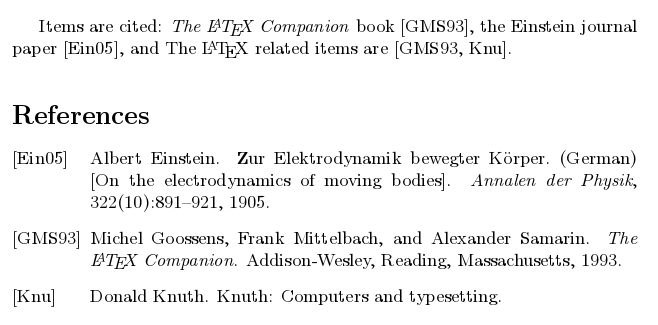
\includegraphics[width=0.8\textwidth]{bibtex-styles-ex-alpha}
  \caption{{\bibtex} output using alpha citation style which uses
    author names and year to index entries.  Source:
    ShareLaTeX~\cite{sharelatex2016_styles}}
\label{fig:bibtex_example_alpha}
\end{figure}


\section{How {\bibtex} is used in practice}
\label{sec:how_bibtex_is_used_today}

To this day, {\bibtex} is routinely used by researchers, witness that
almost all online resources for finding references provide {\bibtex}
output.  Many online databases are widely used to look up entries,
which has also given rise to a variety of ways to identify articles,
such as: arXiv numbers, DOI and ISSN.

Since {\bibtex} is capable of printing only the references used in a
{\LaTeX}-document, most people start using {\bibtex} as a database
having a complete file with the references they have used throughout
time.  A lot of people also find it practical to use their {\bibtex}
file as a way to keep track of what they read.

That {\bibtex} ignores unknown tags is used for de-facto standards, to
add additional information and to comment out tags by prefixing them
with $OPT$.  It is so widely used that is is common to see article
search engines make have tags that are not specified by {\bibtex} and
there is libraries that provide citing styles that make use of these
tags.


\section{Summary and conclusions}
\label{sec:about_conclusion}


{\bibtex} is a product of the advent of {\TeX} and the need for
managing bibliographic references.  The inside of a {\bibtex} file is
simple and intuitive, dividing the entries into types corresponding
to the medium it represents and having tags relevant to that medium.
{\bibtex} has become widely used and given rise to useful de-facto
standards and tools to assist with bibliographic references.

Like {\TeX}, {\bibtex} has been a game changer, and is something for
every scientific author to be happy about.  So has {\bibtex} solved the
problem of bibliographic references? It would seem so, had it not been
for Murphy's Law, as detailed in the next chapter.


%\remark{(Note to self:) should probably have half an eye on things
%  like: `G{\"o}del', when working with it}
%
%\remark{(Note to self:) people may use booktitle where title is
%  appropriate edition: The edition of a book---for example,
%  ``Second''. This should be an ordinal, and should have the first
%  letter capitalized, as shown here; the standard styles convert to
%  lower case when necessary~\cite{bibtex_description}.}
%
%\remark{http://tug2000.tug.org/TUGboat/Articles/tb24-1/patashnik.pdf}f

\chapter{The challenges\\in using {\bibtex}}
\label{ch:problem-description}
\rfquote{Anything that can go wrong, will go wrong.}{Murphy's Law}

\section{Introduction}
The goal of this chapter is to introduce the challenges of {\bibtex}
through concrete examples.  The terms of discourse, structural and
conjunctural, first defined
\chapref{sec:problems_structural_conjunctural}.  The rest of the
chapter is dedicated to problems with: duplicate entries
\chapref{sec:problems_duplicates}, spelling errors
\chapref{sec:problems_spelling}, covering the issues of initials
\chapref{sec:problems_initials}, online lookups
\chapref{sec:problems_look_ups}, name changes of forums
\chapref{sec:problems_name_changes}, de-facto standards and conformity
to the {\bibtex} specification \chapref{sec:problems_de_facto},
journal abbreviations \chapref{sec:problems_abbreviations}, {\bibtex}
strings that end up in the text
\chapref{sec:problems_strings_as_text}, inconsistent tags
\chapref{sec:problems_inconsistent_tags}, and inconsistent entry keys
\chapref{sec:problems_inconsistent_keys} .

\section{Structural vs. conjunctural issues}
\label{sec:problems_structural_conjunctural}

Unfortunately, even though {\bibtex} has made life a lot simpler for
scientific authors, it is far from perfect.  Inspired by economics,
the challenges in {\bibtex} can be divided into \emph{structural} and
\emph{conjunctural} issues.

\begin{itemize}
\item The \emph{structural} issues are the ones intrinsic to
  {\bibtex}: they are caused by its design, its standard tools, and
  missing information in {\bibtex} files.

\item The \emph{conjunctural} issues are the combination of
  circumstances, for instance if the source used does not contain
  complete information (\eg, extracting a reference from an article
  where the authors only have initials even though their full name is
  known) or the users having other practical priorities than assuring
  sound bibliographic references in their scientific writings.
\end{itemize}

Whether an issue is seen as conjunctural or structural is in part a
matter of opinion, as the definitions can be stretched in either
direction -- an issue also faced in economics.  Most of the issues are
arguably a combination of the two: as they could be fixed by careful
labor or by having the right tools available.  For example, most
bibliography managers have tools to switch between abbreviated and
full journal names.

Addressing the human factor, \ie, a conjunctural solution, is one
theoretically possible way for solving these issues.  One option would
be to ``simply'' motivate people to do things right.  Alas people are
not machines and thus this approach will be impossible in practice:
for most people, the interest is not the tools they use, but what they
use them for.  The interest in {\bibtex} is to ensure that their
documents contain appropriately many relevant references.

Since a conjunctural solution is not realistic, the goal is to provide
a structural solution to the issues.  In the perfect world, the
structural solution will be so complete that any issues left will be
entirely conjunctural, because one is either not using or misusing the
structural solution.


\section{Duplicate entries}
\label{sec:problems_duplicates}

When a group of authors is writing on the same document, work is often
divided and each author has their own \file{bib} that they use for
their references.  All might be fine until the group combines their
document and it turns out that multiple authors has used the same
reference, but with different keys, ending up having duplicate entries
in the bibliography.

Arguably it can be seen as a structural or a conjunctural problem.
The similarity of such entries will make them easier to spot with the
naked eye, arguably making a conjunctural solution relevant.  However
due to the similarity (at least if abbreviated the same way), a
structural solution is arguably also easy to make.  Making the problem
purely conjunctural would require a way to detect and merge these
entries.  Furthermore, if the entries use different key names, the
corresponding document should also be corrected. A challenge in this
case is when similar entries, that are still different entries, occur.

A similar issue happened in one of the drafts for this document: when
an author who wants to create a new entry copy and pastes an existing
entry, then giving the new entry an entry key, with intent to adjust
the contents.  This issue will also result in a duplicate entry, but
unlike the situation above, the duplicate should not be merged but
contain different content.

Having a tool that just merges duplicate entries may provide a
structural solution to the first case but will create a structural
issue in the second as it will automatically introduce new issues.
Thus the solution should not merge automatically.


\section{Spelling errors in general}
\label{sec:problems_spelling}

In almost, if not, all cases where people type text, spelling errors
will arise, sooner or later, \file{bib}s are no exception.  Extracting
meta-information automatically from documents may also run into a bad
extraction leading to spelling errors.  Furthermore, a spelling error
might not even be in the {\bibtex} document, as the misspelling can be
from the source, for instance if a title of a document is misspelled,
then the correct {\bibtex} will have to contain this error, as it is
the title of the source.

A user typing the entries manually is arguably the cause of spelling
errors.  Thus it can be argued that the issue is conjunctural, since
one could do a spell check.  However, one might also argue that
{\bibtex} should do a spell check.  In the case where automatic
extraction is the source of the spelling error the tool will give a
structural component to the issue.  Having a way of ensuring a spell
check and if such a way could ensure that the spelling error
corresponds to the source would make this issue conjunctural.


\section{Spelling errors in names}
\label{sec:problems_spelling_names}

Using a spell checker works for most entry tags, except names.  One
citing a name might get the name wrong and write ``Rene Rødhof
Hansen'' instead of ``René Rydhof Hansen''.  In this misspelling the
spell checker will be of no help.  The spell checker used in this
document suggests changing ``René'' to ``Rene'', which would introduce
a mistake.  Using a spell checker on names will be the cause of more
mistakes than corrections, and would thus cause a structural issue.
Providing a structural solution to misspelled names would require
either a spell checker that works for names or some database
containing valid names.


\section{Initials}
\label{sec:problems_initials}

Another issue in \figref{fig:conference_name} is the list of author
names that are so heavily abbreviated to initials that one cannot
realistically distinguish who the authors are.  This might originate
from the used citation style or from a resource where they are already
abbreviated.

If the initials come from the citation style, the issue is of a
structural nature.  However if it is copied from another source, or
just written like that, it is conjunctural, as the user did not ensure
full names.  A structural variant of the copying issue is if the
reference is copied by a tool, then it can be argued that such a tool
should try to detect initials.  Having a way to detect the initials
and the full names will provide a structural solution.  However, to
make an entirely structural solution a reliable way to know when the
initials are deliberate or not is needed.


\section{Online lookups}
\label{sec:problems_look_ups}

Many writers use online lookups for their bibliographic references.
In the Utopic case, all entries can be found online at all times.
Even though the databases out there are really good, erroneous results
can be found.  A lookup on Google Scholar in the beginning of February
2016 for: ``Results and Analysis of SyGuS-Comp’15'' can be seen in
\figref{fig:scholar_bad_result}, which contains an erroneous output.

\begin{figure}
  \centering
\begin{verbatim}
@article{alurresults,
  title={Results and Analysis of SyGuS-Comp’15},
  author={Alur, Rajeev and Fisman, Dana and Singh, Rishabh
          and Solar-Lezama, Armando}
}
\end{verbatim}
  \caption{Bad result from Google Scholar}
\label{fig:scholar_bad_result}
\end{figure}

Having found the article originally on arXiv.org the source of the
article is known to be EPTCS - Electronic Proceedings in Theoretical
Computer Science.  So not only does the Google Scholar result actually
not conform to the requirements of an article, the resource is in fact
not an article at all, but in the proceedings to a conference.
Finding the correct entry details at the EPTCS page reveals the entry
in \figref{fig:eptcs_lookup}.  Relying blindly on these being correct
causes a structural issue since the tools could automatically
introduce new errors.

The entries in those search engines cannot account for unpublished
work either, and expecting all published work to be represented in the
databases would be naive.  Having a reliable way to ensure that all
entries are present, however, is not a likely scenario.

Apart from the desire to detect erroneous entries from bad lookups,
using lookups for suggestions to most of the other issues can be a
useful part of a structural solution.  An optimal structural solution
to the bad lookups would be if it was possible to detect the users'
intended result.  As there is no way to know for certain what the user
intends, this is an Utopian idea.  A realistic idea would be to
provide a solution that limits the risk of bad lookups, which is only
a partial structural solution since the user would still have to
verify the result.

\begin{figure}
  \centering
\begin{small}
\begin{verbatim}
@Inproceedings{EPTCS202.3,
  author    = "Alur, Rajeev and Fisman, Dana  and Singh, Rishabh
               and Solar-Lezama, Armando",
  year      = "2016",
  title     = "Results and Analysis of SyGuS-Comp'15",
  editor    = "\v{C}ern\'y, Pavol and Kuncak, Viktor
               and Parthasarathy, Madhusudan"b,
  booktitle = "{\rm Proceedings Fourth Workshop on}
               Synthesis,
               {\rm San Francisco, CA, USA, 18th July 2015}",
  series    = "Electronic Proceedings in
               Theoretical Computer Science",
  volume    = "202",
  publisher = "Open Publishing Association",
  pages     = "3-26",
  doi       = "10.4204/EPTCS.202.3",
}
\end{verbatim}
\end{small}
  \caption{Correct lookup on EPTCS, after failed lookup on Google Scholar}
\label{fig:eptcs_lookup}
\end{figure}


% ref 3
\section{Name changes of forums}
\label{sec:problems_name_changes}

In \figref{fig:missing_org_scholar_lookup}, spotting the consistency
issues were relatively simple.  When looking at
\figref{fig:entry_journal_name_authors} it can be seen that the
conference name is slightly different in one of the entries, but so
close that they are probably the same conference.

\begin{figure}
  \centering
\begin{small}
\begin{verbatim}
\bibitem{stanifordchen96grids}
S.~S.-C. \emph{et al}.
\newblock {GrIDS} -- {A} graph-based intrusion detection system
          for large networks.
\newblock In {\em Proceedings of the 19th
          National Information Systems Security Conference},
          1996.

[...]

\bibitem{porras97emerald}
P.~A. Porras and P.~G. Neumann.
\newblock {EMERALD}: Event monitoring enabling responses
          to anomalous live disturbances.
\newblock In {\em Proc. 20th {NIST}-{NCSC}
          National Information Systems Security Conference},
          pages 353--365, 1997.

\end{verbatim}
\end{small}
  \caption{Inconsistent reference to the conference and heavily abbreviated author names}
\label{fig:entry_journal_name_authors}
\end{figure}

A visit to the homepage of the conference reveals that ``National
Information Systems Security Conference'' used to be named ``National
Computer Security Conference'', which is probably the reason for the
\texttt{\{NIST\}--\{NCSC\}} part of the first entry~\cite{nist2014_nissc}.  In
the same source it turns out that there are also references to the old
conference name, as seen in \figref{fig:conference_name}, so to
correctly identify potential inconsistencies, it should also recognize
name changes and variations.

\begin{figure}
  \centering
\begin{small}
\begin{verbatim}
\bibitem{snapp91dids}
S.~R.~S. \emph{et al}.
\newblock {DIDS} (distributed intrusion detection system) -
          motivation, architecture, and an early prototype.
\newblock In {\em Proceedings of the 14th
          National Computer Security Conference},
          pages 167--176, Washington, DC, 1991.
\end{verbatim}
\end{small}
  \caption{Name change of a conference}
\label{fig:conference_name}
\end{figure}

In {\bibtex}, there is no way of specifying that the same conference
has different names.  Therefore, there is a big structural part as
there is no support for identifying this issue.  Furthermore, the
owner of the {\bibtex} file might not even be aware of the issue,
which arguably could be conjunctural, since the user could do his
research, or structural, because the user should have a tool that can
assist him.  If a tool could reliably detect inconsistencies from the
same forum with different names, the name changes would become
conjunctural.


\section{De-facto standards and specification conformity}
\label{sec:problems_de_facto}

An interesting point is that not all the structural issues are bad.
There are practical ways to use the relaxed properties of {\bibtex}.
For instance {\bibtex} ignores unknown tags by design which is useful
in de-facto standards such as commenting entries out by prefixing with
$OPT$ or adding information that are not a part of the {\bibtex}
specification, such as ISSN and DOI.  The \texttt{crossref} tag is
technically not specified in {\bibtex}, but is still part of the tool.
In \figref{fig:mendeley_output}, an example is provided by a PhD
student from the Chemistry Department at Aarhus University.  This
example is created from Mendeley (see
Section~\ref{sec:related_mendeley}) and shows a lot of additional
information about the article.

\begin{figure}
  \centering
\begin{small}
\begin{verbatim}
@article{Acatrinei2003,
author = {Acatrinei, Alice I and Browne, D and Losovyj, Y B
          and Young, D P and Moldovan, M and Chan, Julia Y
          and Sprunger, P T and Kurtz, Richard L},
doi = {10.1088/0953-8984/15/33/101},
file = {:C$\backslash$:/Users/[...]pdf},
issn = {0953-8984},
journal = {Journal of Physics: Condensed Matter},
month = {aug},
number = {33},
pages = {L511--L517},
title = {{Angle-resolved photoemission study
          and first-principles calculation
          of the electronic structure of LaSb 2}},
url = {http://iopscience.iop.org/[...]},
volume = {15},
year = {2003}
}
\end{verbatim}
\end{small}
  \caption{Output from Mendeley containing additional information}
\label{fig:mendeley_output}
\end{figure}

This design choice is an issue, if strict conformity to the
specification is desired, as it is practical and widely in use, strict
validation would be counterproductive.  Some formatting styles make
use of unspecified tags, as can be seen in
\figref{fig:entry_with_issn}. It is interesting to find tags that are
not desired, \ie, tags that do not conform to the specification and
the de-facto standards.


%%
%% Internal ref 4
%%
\section{Journal abbreviations}
\label{sec:problems_abbreviations}

Most, if not all, journals require that journal names should be
abbreviated when publishing, especially those from competing
publishers.  However, internally in the {\bibtex} file the owner's
personal priorities are: consistent and correct naming.  As {\bibtex}
can be seen as a database of references, it makes sense to consider
full names as correct and the abbreviations to be a matter of
formatting.  Unfortunately, {\bibtex} does not handle abbreviations at
all, which for instance is apparent in articles from arXiv.org, as can
be seen in the bbl output in \figref{fig:inconsistent_naming}.

\begin{figure}
  \centering
\begin{small}
\begin{verbatim}
\bibitem[\protect\citename{Baroni \bgroup et al.\egroup }2014b]
          {baroni2014don}
          Marco Baroni, Georgiana Dinu, and Germ{\'a}n Kruszewski.
\newblock 2014b.
\newblock Don't count, predict!
          a systematic comparison of context-counting vs.
          context-predicting semantic vectors.
\newblock In {\em Proceedings of the 52nd Annual Meeting of
          the Association for Computational Linguistics},
          volume~1, pages 238--247.

\bibitem[\protect\citename{Bruni \bgroup et al.\egroup}2014]
          {bruni2014multimodal}
          Elia Bruni, Nam-Khanh Tran, and Marco Baroni.
\newblock 2014.
\newblock Multimodal distributional semantics.
\newblock {\em J. Artif. Intell. Res. (JAIR)}, 49:1--47.

[...]

\bibitem[\protect\citename{Collobert \bgroup et al.\egroup}2011]
          {collobert2011natural}
          Ronan Collobert, Jason Weston, L{\'e}on Bottou,
          Michael Karlen, Koray Kavukcuoglu, and Pavel Kuksa.
\newblock 2011.
\newblock Natural language processing (almost) from scratch.
\newblock {\em The Journal of Machine Learning Research},
          12:2493--2537.

[...]

\bibitem[\protect\citename{Kalchbrenner \bgroup et al.\egroup}2014]
          {kalchbrenner2014convolutional}
          Nal Kalchbrenner, Edward Grefenstette, and Phil Blunsom.
\newblock 2014.
\newblock A convolutional neural network for modelling sentences.
\newblock In {\em Proceedings of EMNLP}.
\end{verbatim}
\end{small}
  \caption{Inconsistent naming of journal and conference names}
\label{fig:inconsistent_naming}
\end{figure}

From the point of view that the style of {\bibtex} should format
abbreviations properly, the issue is structural.  In cases where the
abbreviation is wrong (\eg, due to a typo), the issue moves towards
being conjunctural, unless some kind of abbreviation specific spell
checker is being used.  Using full names and then formatting them
accordingly is the most sensible idea, since the style of abbreviation
could be interchanged, should the need arise: it is more readable and
it would create better conditions for output tools to provide
consistent formatting.

Currently there are multiple strategies for ensuring consistency in
abbreviations: some do a search and replace on the \file{bib}.  A bit
more structured one can use the strings in {\bibtex} to ensure a
consistent naming of a journal which can further be combined with the
usage of crossref.  Another approach is the use of Bib{\LaTeX} and
biber Section~\ref{sec:related_biblatex}, which provide the solution
in the formatting options~\cite{koppensteiner2011abbreviate}, provided
that the abbreviation handling of the style is correct.  This solution
causes the formatting issue to become conjunctural.  Bibliography
managers (see Section~\ref{sec:bibliography_managers}) tend to go with
the strategy of storing the references using full names.  When one
using a bibliography manager export to a {\bibtex} file (or another
format), the desired abbreviation style is applied to the export.
This strategy moves the issue towards being conjunctural, for the same
reasons as the Bib{\LaTeX} and biber solution.

As the purpose is to work on the {\bibtex} files, the formatting in
the end is technically not the primary concern.  Optimally the concern
is to ensure a consistent document.  Since {\bibtex} styles do not
take care of abbreviations, there is a need for considerations on how
to deal with consistency and to ensure the desired style of
abbreviations.  A partially structural solution ensures a consistent
structure, which can be modified according to the desired style of
abbreviations.  In a fully structural solution, the styles handle
abbreviations (such as the Bib{\LaTeX} and biber do).


\section{{\bibtex} strings ending up as text}
\label{sec:problems_strings_as_text}

When working with bibliographic references, {\bibtex} strings can
accidentally end up being textual content.  For instance if one, as
the PhD student earlier, exports from a program that does not make use
of the strings.  In the output from the aforementioned student seen in
\figref{fig:mendeley_output} the month is actually a text and not a
string as one would expect.  The use of text over strings prevents
re-use of fragments and localization.

When the usage as text over strings comes from a tool, such as in the
example above, the issue is of a structural nature.  When one types it
by accident then again it can arguably be both structural and
conjunctural.  Providing a structural solution to this would be by
being able to detect this and correct it.


%%
%% Internal ref 1
%% journal unknown oO
%%
\section{Inconsistent tags}
\label{sec:problems_inconsistent_tags}

Take the inconsistency in \figref{fig:entry_with_issn}, found in an
article on arXiv.org: two references from the same conference, but
with different years.  The inconsistency is easy to identify due to
the consistent content.  Correct and consistent content will help
tools in detecting inconsistencies.  This exposes a structural part of
the issue, as no such tools exist (to the authors' knowledge).

\begin{figure}
  \centering
  \begin{small}
\begin{verbatim}
\bibitem[Bernardy and Claessen(2015)]{bernardy_efficient_2015}
J.-P. Bernardy and K.~Claessen.
\newblock Efficient parallel and incremental parsing
          of practical context-free languages.
\newblock \emph{J. of Funct. Prog.}, 25, 2015.
\newblock ISSN 1469-7653.
\newblock \doi{10.1017/S0956796815000131}.

[...]

\bibitem[Mu et~al.(2009)Mu, Ko, and Jansson]{MuKoJansson2009AoPA}
S.-C. Mu, H.-S. Ko, and P.~Jansson.
\newblock Algebra of programming in {Agda}:
          dependent types for relational program derivation.
\newblock \emph{J. Funct. Program.}, 19:\penalty0 545--579, 2009.
\newblock \doi{10.1017/S0956796809007345}.
\end{verbatim}
  \end{small}
  \caption{Additional tag ISSN is provided in one of the entries}
\label{fig:entry_with_issn}
% consider the pages
\end{figure}

The ISSN might not exist for the \texttt{MuKoJansson2009AoPA}-entry.
In this case a structural detection system might be the cause of new
structural issue, either the removal of relevant data or forcing
entries when the data does not exist.  In this specific case, the
search result in \figref{fig:entry_issn_found} reveals that the
missing ISSN does exist and thus a tool pointing out the inconsistency
would in this case make the issue conjunctural.

% Source http://journals.cambridge.org/action/displayAbstract?fromPage=online&aid=6171388&fileId=S0956796809007345#
\begin{figure}
  \centering
\begin{verbatim}
@article{Mu:2009:APA:1630623.1630627,
 author = {Mu, Shin-cheng and Ko, Hsiang-shang
           and Jansson, Patrik},
 title = {Algebra of Programming in Agda:
          Dependent Types for Relational Program Derivation},
 journal = {J. Funct. Program.},
 issue_date = {September 2009},
 volume = {19},
 number = {5},
 month = sep,
 year = {2009},
 issn = {0956-7968},
 pages = {545--579},
 numpages = {35},
 url = {http://dx.doi.org/10.1017/S0956796809007345},
 doi = {10.1017/S0956796809007345},
 acmid = {1630627},
 publisher = {Cambridge University Press},
 address = {New York, NY, USA},
 }
\end{verbatim}
  \caption{Search revealing the ISSN}
\label{fig:entry_issn_found}
\end{figure}

%%
%% Internal ref 2
%% Source Electronic Proceedings in Theoretical Computer Science
%%

Provided a reliable way to lookup correct entries, a tool could move
the issues towards being conjunctural.  Take the inconsistency in
\figref{fig:inconsistent_proceedings} where two entries from the same
conference have different information.  One has an additional ``ICFP
'10'' and ``ACM'' in there, the other one does not.

\begin{figure}
  \centering
  \begin{small}
\begin{verbatim}
\bibitem[Bernardy and Claessen(2013)]{bernardy_efficient_2013}
J.-P. Bernardy and K.~Claessen.
\newblock Efficient divide-and-conquer parsing
          of practical context-free languages.
\newblock In \emph{Proc. of ICFP 2013}, pages 111--122, 2013.

[...]

\bibitem[Danielsson(2010)]{danielsson_total_2010}
N.~A. Danielsson.
\newblock Total parser combinators.
\newblock In \emph{Proc. of ICFP 2010}, ICFP '10,
          pages 285--296. ACM, 2010.
\end{verbatim}
  \end{small}
  \caption{Capt}
\label{fig:inconsistent_proceedings}
\end{figure}

An online search for {\bibtex} information gives the entries in
\figref{fig:missing_org_scholar_lookup} for the two articles, which
provides one possible option for a set of consistent entries.  As can
be seen, $ACM$ is the name of the organization and is probably missing
in the original {\bibtex} that produced the \file{bbl} inspected
above.  The Danielsson has additional information with the content
``ICFP '10'', which is not apparent in the search result.

\begin{figure}
  \centering
\begin{verbatim}
@inproceedings{bernardy2013efficient,
  title={Efficient divide-and-conquer parsing
         of practical context-free languages},
  author={Bernardy, Jean-Philippe and Claessen, Koen},
  booktitle={ACM SIGPLAN Notices},
  volume={48},
  number={9},
  pages={111--122},
  year={2013},
  organization={ACM}
}

@inproceedings{danielsson2010total,
  title={Total parser combinators},
  author={Danielsson, Nils Anders},
  booktitle={ACM Sigplan Notices},
  volume={45},
  number={9},
  pages={285--296},
  year={2010},
  organization={ACM}
}
\end{verbatim}
  \caption{Scholar lookup}
\label{fig:missing_org_scholar_lookup}
\end{figure}

\section{Inconsistent entry keys}
\label{sec:problems_inconsistent_keys}

The naming scheme for entry keys may vary throughout a \file{bib}.
For example, one of the users collaborating earlier might use entries
from various online databases getting keys corresponding to
\figref{fig:missing_org_scholar_lookup}, \figref{fig:eptcs_lookup} and
other structures in one big mess.  One of the users collaborating
might also be new to using {\bibtex} (could be a student learning) and
needs to find a nice an consistent way of writing the keys.

A challenge could be to avoid duplicate key names, which with a
consistent structure is more likely.  The duplicate entry keys can
have the advantage that it can be an indicator of a duplicate entry
Section~\ref{sec:problems_look_ups}.

Inconsistencies in keys might range from not a problem at all to fully
conjectural or structural, highly depending on the one's point of
view.  A user may simply not care and apart from the potential to
detect duplicate entries, may not feel a reason to.  In the
collaboration scenario, the additional way of detecting duplicates may
be valuable.  In this case, it arguably becomes conjunctural since the
authors should have agreed on a style - which might also have helped a
newcomer to have a good practice.  It can also be argued that it is
structural since {\bibtex} does not provide naming guidelines nor
tools for ensuring a guideline.

To make this issue structural, a naming convention would have to be
specified and some way of detecting deviations provided.  A blind
application of this method could result in two entries colliding with
the same key, requiring the attention of the user.


\section{Summary and conclusions}
\label{sec:problems_conclusion}

{\bibtex} has a lot of issues, for which a structural solution is
desired.  The problems covered are:

\begin{itemize}
\item Duplicate entries are not desired.  A structural solution will
  be to detect and merge duplicates, because a duplicate originating
  from missing or wrong data automatically merging may cause issues.

\item Spelling errors in general.  A structural solution will be able
  to find and correct the spelling errors, preferably by having the
  same spelling as published.  Alternatively, running a spell checker
  and having a way to account for deliberate misspellings, domain
  specific words and choice of language.

\item Spelling errors in names will challenge normal spell checkers.
  A structural solution is a spell checker that works for names or a
  database with names to verify names.

\item Use of initials can hide people's names to the level where
  finding a resource is hard.  A structural solution is to detect
  initials and the full names, accounting for when the initials are
  deliberate.

\item Online lookups can contain wrong data.  Optimally we can detect
  these wrong data reliably: the most realistic idea is to provide a
  way that limits the likelihood of erroneous results.

\item Name change of a forum which can affect detection of
  inconsistent tag use.  A structural solution will have some way of
  detecting when sources are from the same forum.

\item Conformity to de-facto standards and the {\bibtex} specification
  is desired, but should not prevent new de-facto standards.  A
  structural solution requires something that checks the conformity to
  a combination of specifications and de-facto standards accounting
  for changes in de-facto standards.

\item Journal abbreviations can be an issue for analyzing tools and
  having full names in {\bibtex} files.  A structural solution will be
  able to ensure that all entries are consistently abbreviated or
  de-abbreviated, preferably accounting for that people may want to
  switch between for formats.

\item {\bibtex} strings that end up as part of the text, can result in
  wrong data.  A structural solution will be able to detect and make
  text into strings when a string is desired.

\item Inconsistent tag usage in similar entries causes messy
  bibliographies. A structural solution will detect these
  inconsistencies and will be able to suggest a course of action.
  This solution may be challenged by deviations in information and
  forums that change name.

\item Inconsistent entry keys which can be an issue in collaboration
  and may make it harder to detect duplicates.  A structural solution
  could be to apply a naming scheme for the entry keys, accounting for
  similar entries that would result in identical entry keys.
\end{itemize}

With all these problems at hand, {\bibtex} may not seem like the
optimal tool after all.  What can be done with such a range of
issues?


\chapter{Our approach to {\bibtex}}
\label{ch:approach}
\section{Introduction}
The goal of this chapter is to organize the issues people have with
{\bibtex}.  Answering what the issues in {\bibtex} are
\chapref{sec:intro_what_issues} and how to approach the {\bibtex}
issues \chapref{sec:intro_what_to_do}

\section{What are the issues in {\bibtex}}
\label{sec:intro_what_issues}

{\bibtex} has changed the landscape for scientific writing and eased a
lot of people's lives, however not without any issues.  The challenges
range widely and trying to group similar looking issues we have:

The misspellings in general, misspellings in names, initials in author
names, use of abbreviations for journal names, and {\bibtex} strings
that end up being text will be considered as lexical concerns.
Conforming to the specification and de-facto standards is considered
as a correctness concern.  All of these issues will be considered
combined as \newdef{correctness and lexical concerns}.

Duplicate entries, forum names that change, inconsistent use of tags
and inconsistent entry keys will be considered as \newdef{consistency
  concerns}.

The Utopian goal is to provide a structural solution for all these
issues so that if any further issues exist they would be purely
conjunctural.


\section{What can be done about the {\bibtex} issues}
\label{sec:intro_what_to_do}

As previously stated, the structural approach to the issues is desired.
This choice basically means ensuring that the tools handle the
issues, preferably to the level where all issues are solved.  As
touched upon shortly when inspecting the problems, it is not likely
that all issues can be solved perfectly.  For a structural solution
there are two approaches:


\subsection{Updating or replacing {\bibtex}}

One way of handling the issues structurally would be to change or
replace {\bibtex}, so it handles all lexical and consistency concerns.
This way would include changing the {\bibtex} specification to account
for relevant de facto standards, enforcing conformity, handling
abbreviations and controlling all data.  The updated version of
{\bibtex} could then either correct the issues when running into them
or fail building the \file{bbl} with appropriate error messages for
issues that the user needs to take care of.

This approach would be probably be perceived as invasive as it would
cause existing {\bibtex} files not to work and it would impose the
tool on the users with requirements they may not desire.  The
perception would of course depend on perspective because the user who
wants structure and control might find it good that it is enforced.

As will be inspected in Chapter~\ref{ch:related} there are actually a
few attempts at both changing and replacing {\bibtex}.


\subsection{Augmenting {\bibtex}}

Instead of changing or replacing {\bibtex} an augmenting tool is
another option.  Such a tool can be used together on {\bibtex} file
to provide or suggest improvements, instead of changing specifications.
An augmenting tool will be a supplement to current use of {\bibtex}
and be optional, rather than imposed on the users.


\section{How do we approach the {\bibtex} issues}
\subsection{Introduction}

The goal of this section is to introduce our choice of solutions for
the issues.


\subsection{Lexical and correctness concerns vs. consistency concerns}
\label{sec:approach_lexical_consistency}

The relation between the lexical and correctness concerns and the
consistency concerns reveals a dependency in the analysis.  Going
through the consistency concerns observing their relation gives:

\begin{itemize}
\item For inconsistent use of tags, a way to determine if entries are
  from the same forum is needed.  Such a way depends on consistent
  naming of the forum and a way to detect name changes.

\item For duplicate entries having unique identifiers such as arXiv
  numbers, ISSN or DOI will make the detection trivial.  Otherwise the
  detection has to be based on the similarity of the information.  At
  best the information is identical, otherwise it has to be as similar
  as possible to improve the detection.  Thus solving the lexical
  concerns will be of use.

\item Inconsistent naming of entry keys can be handled by a naming
  scheme.  Such a naming scheme is usually based on the information in
  the entries.  So having the relevant tags and correct content in
  them will provide a way to ensure consistent entry keys.

\item For name changes of forums we need to be able to recognize the
  names which is easier with correct and consistent names.
\end{itemize}

A common property about the consistency concerns is that they are
easier to handle, once the lexical and correctness concerns have been
handled.  This property indicates that a two phase solution may be
desired: first handling the lexical and correctness concerns, then
handling the consistency concerns.


\subsection{\nameref{sec:problems_duplicates}}
\label{sec:approach_duplicates}

Duplicate entries are fairly straight forward if the tags and the
contents are identical.  If the content and tags deviate a way to
detect ``similarity'' will be needed.  The easiest definition of
similarity is if the title and author is identical, however this
definition might need to take things like revisions and year into
account, as an author may decide to write a new version later or if
one for some reason desires to refer to different revisions.  Further
challenges may arise if there is lexical and correctness challenges as
per Section~\ref{sec:approach_lexical_consistency} fixing these first
is desired.


\subsection{\nameref{sec:problems_spelling}}

To detect misspellings a spell checker can be used.  Alternatively
checking the resources in online databases is an option.  If a spell
checker is used one should be aware of false positives.  Domain
specific terms might not be present in the dictionary and if the
original source is misspelled, it would be a mistake to correct it
(once published the name published is the correct name of the
reference!).  Provided a solution for the issues in online look ups
the correct spelling will be a matter of looking up, but references
may not be in the databases, and as stated in
Section~\ref{sec:approach_look_ups} there is no good way to ensure
correct look ups.  So a spell checker seems like a good way to get an
indication of possible errors, but one would still have to verify
them.  As entries may be in different languages a way of specifying
the language should be considered.


\subsection{\nameref{sec:problems_spelling_names}}
\label{sec:approach_spelling_names}

Spell checking names with a normal spell checker will cause errors.  A
possible way to approach this would be to make online look ups in
databases with scientific authors, such as DBLP and Google Scholar.
This will still have the issue with name of authors who have not
published anything scientific.  Extending this solution to contain
more databases such as book authors will improve the solution, but
will still be limited to known author names.


\subsection{\nameref{sec:problems_initials}}

Finding the initials is a matter of being able to detect single
letters with or without a period after it.  However if one for some
reason groups initials together, \eg, making George R. R. Martin into
George RR Martin, then further detection will be needed.  Replacing
the initials with full names is appropriate whenever possible, but
since the full names may not be known some way of specifying that
initials is the only thing available is needed.  The best approach
will probably be the one described for spell checking names in
Section~\ref{sec:approach_spelling_names}.


\subsection{\nameref{sec:problems_look_ups}}
\label{sec:approach_look_ups}

Online database look ups can be a very useful tool for handling the
lexical and correctness concerns, but getting incorrect data can cause
problems.  The best approach to ensure correct look ups is if it is
possible to use services that are known to be correct.

A situation where relatively reliable look ups is possible, as in the
``EPTCS'' look up seen in \figref{fig:eptcs_lookup}, can be used to
improve the reliability of the results.  However there is still no
certain way to know if the database of the service is correct, so it
is still not certain.  Most likely the ID systems, such as arXiv
numbers, DOI and ISSN, will also provide a relatively reliable look up
mechanism, but it is still not guaranteed.

Another way to approach the bad look ups could be by doing the same
look up in multiple databases and then have some kind of voting system
that decides on which entry to trust.  This would however require
knowledge information sources each online service use, because their
source of information may be the same and then the same error could
get multiple votes.  The approach can be refined by having increased
trust in databases that are likely to be correct.

The most appropriate strategy is probably selecting the database most
likely to be correct and then have the user select if one agrees with
the result.  Doing the vote system would be overkill in most
situations, and the user still has to validate the result, since the
voting system will not provide a certain correct result.  Having the
user validate the result will make issues partly conjunctural, if one
just accept any result from the look up.


\subsection{\nameref{sec:problems_name_changes}}

Handling name changes of forums is supportive to ensuring consistency.
Since name changes cannot be derived automatically one approach would
be a database of known name changes, which has the disadvantage that
it needs to be maintained.  Adding a configuration to specify name
changes may also be appropriate.


\subsection{\nameref{sec:problems_de_facto}}

As stated in Section~\ref{sec:problems_de_facto} it is desired to be
able to validate if the file conforms to the specification and the
desired de-facto standards.  Validating conformity to the
specification is a simple task, as the specification is just a set of
rules.  A set of de-facto standards, likewise, is also a simple set of
rules.

De-facto standards however provide challenges, as they are the
standards currently in use.  This means that they both depend on who
the user is and the standards are subject to change.

A tool handling conformity to the specification and de-facto standards
should thus be configurable to account for changes in de-facto
standards.  For practicality the de-facto standards that are not
likely to change (such as ISSN and DOI) could be accounted for with a
default setting.


\subsection{\nameref{sec:problems_abbreviations}}

Ensuring a consistent use of either abbreviations or full names is
desired.  From the point of having the information in a complete
version converting full names, \newdef{de-abbreviating} is desired.
Using a database of standard abbreviations for forums will be useful
to de-abbreviate.  Taking care of a consistent way to switch between
full names and abbreviations is also desired.  Making use of strings
to handle the switching between full names and abbreviations is
probably the best approach since this will keep it clear which forum
is which.  This also allows the user to use string names that are:
full names, official names or their own style of abbreviations, to
their choice.


\subsection{\nameref{sec:problems_strings_as_text}}

A {\bibtex} string can end up being part of a text by mistake.  In the
example used in Section~\ref{sec:problems_strings_as_text} where the
month ended up as a text rather than a string a simple check is
possible, because for a month we know what to expect.  Whenever
something in the middle of the text should have been a string, the
text would have to be checked for potential strings.  Automatically
correcting it would introduce a potential source of errors, because a
text being identical to a string name could just be a coincidence, so
it has to be the user's choice.


\subsection{\nameref{sec:problems_inconsistent_tags}}

Detecting inconsistent use of tags requires a way of detecting when
entries are from the same forum.  When such a way is provided it is
possible to check if the set of fields are the same.  Having some kind
of statistics on the usage may further improve the feedback, since it
will be possible to suggest the shortest path to consistency: if it is
by adding, or removing tags.

Since a lot of the forums are continuous, such as a conference being
held each year, the detail level of the information may change over
time.  Also in some cases a single item can have additional
information that is not general to the forum or for some reason not
have information according to the general standard.  Optimally there
should be a way to account for these cases, either by the user
enforcing conformity or having options for when a deviation occurs.


\subsection{\nameref{sec:problems_inconsistent_keys}}

Provided that the lexical and correctness concerns have been solved,
handling inconsistent entry keys require very little effort.  Having a
rule for how the key names should be formatted is all that is needed.
Like in Section~\ref{sec:approach_duplicates} there is the issue of
similar, but different, entries.  Similar entries could result in the
same entry key, so there is the need for a way to disambiguate the key
names.  Since a lot of users already have databases in use, support
for one specifying a naming scheme would be appropriate.


\section{Summary and conclusions}

The issues in {\bibtex} files have been grouped in correctness and
lexical concerns and in consistency concerns.  Updating or replacing
{\bibtex} was compared to augmenting {\bibtex}.  It was observed that
the consistency concerns in general depend on the solution of the
correctness and lexical concerns.

\begin{itemize}
\item Duplicate entries can be found if there is a unique identifier
  or identical entries.  To detect deviating duplicates a definition
  of ``similarity'' will be needed.

\item Spelling errors in general can be solved by a spell checker and
  the usage of online look ups.  For a spell checker one must be aware
  of false positives and language.

\item Spelling errors in names will challenge normal spell checkers.
  Using online databases of authors will enable some checking but the
  solution will be limited to known author names.

\item Initials hiding people's names can be handled by online
  resources, just as misspellings in names.

\item To get online look ups that contain the correct data is
  impossible, the results can be improved by selecting the most
  appropriate database for the look up and by introducing detection of
  erroneous look ups.

\item Name change of a forum can be handled by a database and by a way
  to specify name changes.

\item Conformity to de-facto standards and the {\bibtex} specification
  should be handled by checking the rules for the standards and being
  able to specify the desired de-facto standards.

\item Journal abbreviations should be moved into strings and be
  consistently de-abbreviated or abbreviated.

\item {\bibtex} strings that end up as part of the text should be
  detected by matching string names that appear in text.

\item Inconsistent tags should be detected based on when entries are
  from the same forum.  One should be able to specify deviations from
  the general set of information for the forum.

\item Inconsistent entry keys should be handled by a rule for the
  desired format for entry key names.
\end{itemize}

Handling the {\bibtex} issues will be done by augmenting {\bibtex}
with a multiple phase tool.  The tool will address the correctness and
lexical concerns first, then the consistency concerns.


%\begin{figure}
%  \centering
%  \begin{verbatim}
%This is BibTeX, Version 0.99d (TeX Live 2015/Debian)
%The top-level auxiliary file: doc.aux
%The style file: plain.bst
%Database file #1: mybib.bib
%Warning--can't use both author and editor fields in book
%Warning--empty publisher in book
%Warning--empty year in book
%Warning--empty journal in Nobody06
%Warning--empty year in Nobody06
%\end{verbatim}
%  \caption{Example of error output from {\bibtex}}
%\label{fig:bibtex_out}
%\end{figure}


%\remark{People who request similar
%http://stackoverflow.com/questions/13630584/the-best-method-for-handling-bibtex-files
%http://stackoverflow.com/questions/32838020/awk-how-to-clean-bibtex-files
%http://www.latex-community.org/forum/viewtopic.php?f=50&t=12043
%http://tex.stackexchange.com/questions/76420/cleaning-up-a-bib-file
%http://tex.stackexchange.com/questions/174509/is-there-a-tool-service-that-can-enrich-a-bibtex-database
%<http://tex.stackexchange.com/questions/128989/how-can-one-validate-a-bib-file
%http://tex.stackexchange.com/questions/173621/how-to-validate-check-a-biblatex-bib-file
%http://stackoverflow.com/questions/13630584/the-best-method-for-handling-bibtex-files
%}


%%% Local Variables:
%%% mode: latex
%%% TeX-master: "thesis"
%%% End:


\chapter{Related work}
\label{ch:related}
\section{Mendeley}

%%% Local Variables:
%%% mode: latex
%%% TeX-master: "thesis"
%%% End:


\chapter{Analyzing {\bibtex} files}
\label{ch:analyzing}
\rfquote{Testing shows the presence, not the absence of bugs.}{Edsger
  W. Dijkstra}


\section{Introduction}

The goal of this chapter is to show how {\bibtex} files are analyzed.
Covering: what should be done about {\bibtex} in principle and
practice \chapref{sec:analyzing_what_to_do} and an analyzing prototype
named {\orangutan} \chapref{sec:analyzing_orangutan}.


\section{What should be done about {\bibtex}}
\label{sec:analyzing_what_to_do}
\subsection{In principle}

Due to the practical issues in changing/replacing {\bibtex} and to
ensure separation of concerns an analyzing tool should be an
augmenting tool.

To analyze {\bibtex} one would need to parse a {\bibtex} file into a
suitable representation.  This representation would need to parse
{\bibtex} entries and strings at a minimum.  If one intents to pretty
print the result after resolving all issues, the parsing also needs
the preambles.  Comments are technically optional, but should be kept
too.

The easiest approach is a two step parse: first taking care of the
lexical and correctness concerns, then the consistency concerns.  By
taking care of the lexical and correctness concerns first the optimal
conditions for taking care of the consistency concerns is made.

The term database i here use for both local and online databases,
since it does not matter if one use a local copy, if it is up to date.

\subsubsection{First step: Lexical and correctness}
\begin{itemize}
\item Spelling errors in general, should be detected either by online
  lookups or a spell checker.  A combination of the two could be
  powerful, since it gives a potential indicator of false positives.
  Using a spell checker requires a way to configure the language for
  the individual entries.

\item Spelling errors in names should use databases with names for
  detection.

\item Initials can be detected by finding cases with a single letter,
  perhaps followed by a punctuation.  For suggestions databases with
  names will be useful.  Handling multiple letters combined can be
  done by looking for relatively few (probably up to 3) letters that
  are all capitalized.

\item Online lookups, will be impossible to detect for certain,
  because the intended search will be unknown.  The detection of the
  other issues can give an indicator of a bad lookup.  Since online
  lookups is a likely way to handle the databases needed for this
  tool, the quality of a lookup is a concern.  The most trusted online
  database available should be used whenever possible.  A system doing
  lookups in multiple databases will give further indications of
  potential issues.  The results should always be confirmed by the
  user, to prevent erroneous data.

\item Conformity to de-facto standards and the {\bibtex} specification
  requires a set of rules specifying: required tags, optional tags,
  exclusive tags, and inclusive tags.  The values should be validated
  to the extend possible.

\item Detecting invalid values should be done where there are clear
  rules for a correct value can be specified: such as ISSN, year, and
  month.  Furthermore, values that can be verified using a database
  should also be verified.

\item To detect journal names, in abbreviated form, or in full form,
  is done using a database of know journal names and their
  abbreviations.  It should use a database to de-abbreviate or
  abbreviate.  Furthermore this can be refined by detecting unknown
  abbreviations.

\item To handle {\bibtex} strings that end up as part of the text, the
  text should be compared with the strings in the \file{bib}.
\end{itemize}


\subsubsection{Second step: Consistency}
\begin{itemize}
\item To detect duplicate entries, using unique identifiers is the
  best way, then based on identical entries.  Otherwise potential
  duplicates is detected by a specification of similarity: having the
  title and authors as primary indicators.  For duplicated values it
  should use the strings if possible to determine when the same source
  is referenced.  For the duplicated values is should build a list of
  values that are likely to be repeated (such as journal names) and
  use that to detect when textual content are duplicated.

\item To detect name changes of forums, a database of known changes is
  used, in conjunction with a way of specifying the changes.

\item Inconsistent tag usage should be handled by mapping entries from
  the same forums and comparing the tags in use for missing and
  additional tags.  Comparing forum entries over time will increase
  the usefulness, but adds the need to handle changes in the tags in
  use over time.

\item Inconsistent entry keys should be handled by having a naming
  scheme based on the data in the entries, with a way to disambiguate
  if two different entries would get the same name.
\end{itemize}


\subsubsection{Configuration}
\label{sec:analyzing_configuration}

Both of the steps above require ways to configure the behavior, to
prevent false positives.  The use of configurations should be as close
to {\bibtex} as possible.

The preference to using the {\bibtex} format allows people to use what
they are familiar with.  Using a format that are readily supported in
programming frameworks, like JSON or XML might be considered easy by
the computer scientist, especially if it is one used to working with
those formats.  However, people outside computer science, such as a
physicist or the helpful chemist from earlier, will likely not be
familiar with such formats, nor should they.  A user of {\bibtex}
should at best only be concerned with {\bibtex}, when working with
{\bibtex}.

To use something in anger is an idiom for if something has been tested
in practice.  The idea of coding in anger has been expressed by Philip
Wadler~\cite{wadler1997_functional}.  For the {\bibtex} user, coding
in anger, could be the situation where the deadline is getting closer
and one just need things to work, at best ten minutes ago.  When faced
with the frustrations like that one tend not to care about beautiful
and elegant solutions, but rather wanting something that works with a
minimum of effort.  To accommodate the user writing {\bibtex} in
anger, is another reason to keep the specification as close to
{\bibtex} as possible, since it will minimize the effort.

Configuration should be done via de-facto standards inside the
\file{bib}, whenever possible.  For some configurations, de-facto
standards inside the \file{bib} is unreasonable.  These configurations
is better put into separate files.  However, the specification of
should still be designed to match {\bibtex} as closely as possible,
\ie, still using entries, tags and values to configure.


\subsection{In practice}
\label{sec:analyzing_in_practice}

\subsubsection{Entry level configurations}

To account configure the analysis, introducing two de-facto
standards will be appropriate: \texttt{OLDforum} to mark a previous
name of a forum, and \texttt{OPTanalyze} to configure tell the tool
about entry specific details.

The division into two de-facto standards are done for two reasons: for
\texttt{OLDforum} the additional standard will allow bibliography
styles to make use of the additional information (one could easily
imaging a bibliographic style write ``\texttt{NISSC \textit{formerly
    known as} NCSC}''), and for \texttt{OPTanalyze} the content is
considered unlikely to be relevant to print in a bibliography.
Furthermore, the settings for \texttt{OPTanalyze} is kept in one tag
to prevent a multitude of new tags.

\remark{Olivier: Yikes, is there any way to make the following
  clearer?}

For the \texttt{OLDforum} tag, the value should be the string
containing the old name for the forum.  In some cases a forum can have
multiple name changes.  When multiple name changes occurs, referring
the most recent name in the \file{bib} is desired.  The tag is
intended for disambiguation within a given file, not all files in
general.  If the tag is used for a bibliography style having a
multitude of names as the value will likely be confusing.

However, if a forum name has been omitted, because no entries with
that name was in the \file{bib}, then a re-detection of name changes
will be needed if this name is added later.  Furthermore, using it in
bibliography styles may cause issues if we only desire to show the
previous name, when it is used in the references, however, since the
tag is presently not in use in any bibliography style, these issues
are not considered further.  Alternatively the format could be a list
of names (comma separated, since {\bibtex} use a comma as a
separator), this list would allow detailed backtracking.  A design
with detailed backtracking

Defining entry level deviations is done using \texttt{OPTanalyze},
using spaces to separate multiple settings.  The values for desired
deviations is as follows:

\begin{itemize}
\item \texttt{@DUPLICATEOK=X} to specify that an entry marked as a
  potential duplicate if deliberate, replacing \texttt{X} with the
  entry key of the potential duplicate.
\item \texttt{@LANG=XX} to specify the desired spell check language,
  replacing \texttt{XX} with the language code desired.
\item \texttt{@SPELLINGOK} to mark the spelling as correct.
\item \texttt{@NAMESOK} to mark that the names are correct.
\item \texttt{@INITIALSOK} to mark that the initials are correct.
\item \texttt{@NOLOOKUP} to mark that no look up should be done for
  the content of this entry.
\item \texttt{@CONFORMITYOK} to mark conformity to the specification
  and de-facto standards as correct.
\item \texttt{@ABBREVIATIONOK} to mark an abbreviated form as correct.
\item \texttt{@STRINGSOK} to mark that the texts has been checked for
  strings and that is is correct.
\item \texttt{@TAGSOK=forum} to mark that the usage of tags is correct and
  defines the standard for tag use for the entries from the \emph{same
  occurrence} of the forum.
\item \texttt{@TAGSOK=future} to mark that the usage of tags is
  correct and defines the standard for tag use for the entries from
  the \emph{same and future occurrences} of the forum.
\item \texttt{@TAGSOK=single} to mark that the usage of tags is
  correct for this single entry, not affecting other entries from the
  forum.
\item \texttt{@ENTRYKEYOK} to mark the entry key as correct.
\item \texttt{@LEXICALLYOK} to ignore all lexical checks for the
  entry.  Should be used with care.
\item \texttt{@CONSISTENCYOK} to ignore all consistency checks for the
  entry.  Should be used with care.
\item \texttt{@OK}, to mark an entry as fully correct, essentially the
  same as marking the entry with: ``\texttt{@CONFORMITYOK @LEXICALLYOK
    @CONSISTENCYOK}''.  Should be used with care.
\end{itemize}

The settings: \texttt{@ABBREVIATIONOK}, \texttt{@LEXICALLYOK},
\texttt{@CONSISTENCYOK}, and \texttt{@OK} may be a bit debatable on
necessity, however, their presence do ensure that the configuration is
complete and consistent.

For the conformity and de-facto analysis, a consideration would be to
have configurations, for explicitly specifying explicitly specifying
that which deviations that are being accepted.  For instance,
specifying that we accept a missing title on one of the articles.
However, explicitly allowing and denying tags will likely be
redundant, since once the deviation has been accepted one will not be
likely to change that.

A similar set of tags could also be defined for the consistency check.
For the consistency check, it can be argued that an entry not
conforming to the standards of a forum may be updated to do so.  For
instance, if the norm for a forum is to have an ISSN on all entries,
and some of the entries do not have an ISSN.  Those entries might get
an ISSN assigned later, which we at the time add to the entry.  In the
case of adding the missing information, the \texttt{@CONSISTENCYOK}
configuration will become redundant.  By knowing which tags caused the
addition of \texttt{@CONSISTENCYOK}, one can remove the redundant
configuration.  Another approach to configurations becoming redundant
is to analyze whether the configurations have any effect on the
analysis.  This approach is considered more appropriate, because of
the simplicity for the user.

Another potential change is: to have a configuration for trusted
lookup services.  For example, if one knows that an entry is correct
in a certain database, then specifying that this database is trusted
for that entry.  This configuration might lead to a false sense of
security, since there is no way to guarantee that the data will never
be corrupted in that database.

An example of the configurations can be seen in
\figref{fig:analyzing_added_de_facto_standards}

\begin{figure}
  \centering
\begin{verbatim}
@BOOK{blendstrup1994Mistbaenk,
  author = "Jens Blendstrup",
  title = "Mennesker i En Mistb{\ae}nk",
  year = 1994,
  OPTanalyze = "@LANG=DA @NAMESOK @CONFORMITYOK"
}
\end{verbatim}
  \caption{An example using the de-facto standards for configuration,
    setting the spell checking language to Danish, accepting the name
    ``Jens Blendstrup'' and ignoring the missing publisher.}
  \label{fig:analyzing_added_de_facto_standards}
\end{figure}

To make the configurations even more intuitive for a {\bibtex} user,
an option is to add {\bibtex} strings with the relevant options in the
top of one's \file{bib}.  Then when configuring one can just use the
{\bibtex} strings and concatenate the relevant configurations.  An
example of configuration with strings can be seen in
\figref{fig:analyzing_added_de_facto_standards_strings}.  These
strings would then have to be added in the top of the \file{bib}, so
{\bibtex} will not complain.

\begin{figure}
  \centering
\begin{verbatim}
@BOOK{blendstrup1994Mistbaenk,
  author = "Jens Blendstrup",
  title = "Mennesker i En Mistb{\ae}nk",
  year = 1994,
  OPTanalyze = analyze_lang_danish
             # analyze_names_ok
             # analyze_conformity_ok
}
\end{verbatim}
  \caption{\figref{fig:analyzing_added_de_facto_standards_strings}
    rewritten to use strings for configuration.}
  \label{fig:analyzing_added_de_facto_standards_strings}
\end{figure}


\subsubsection{Bibliography level configurations}

For the configurations desired, some are not specific to an entry, but
rather the entire bibliography.  Two options for these configurations
are: to put such options inside one's \file{bib}, or put them in
separate files.  Adding them to one's \file{bib} will introduce an
additional mess in the file, which is counterproductive since the goal
is to clean up the mess.  Furthermore, the configurations may not
correspond to proper {\bibtex} formatting.  Having the configurations
in separate files, provides: separation of concerns, a clean
\file{bib} and allows deviations from {\bibtex} if needed.
Furthermore, having configurations in separate files allows sharing of
the files, for instance, if a publisher want their authors to follow a
certain setup.

Such configuration files should still, if possible, follow the
{\bibtex} format.  Thus using entries with tags and values for
configuration and for configurations where entries and tags do not
make sense, defining {\bibtex} strings will be the favored choice.

Because the format described can be put into one file, rather than
many, there are a few issues with disambiguation.  For instance, there
can be multiple configurations for the title of a
\texttt{@PROCEEDINGS}.  To solve this then the first word in the entry
keys identify the type of configuration, followed by an underscore and
a descriptive name of the user's choice.  For example the key
\texttt{forum\_ncsc}, seen in
\figref{fig:analyzing_configuration_name_change}, indicates that the
configuration is regarding the forum (more specifically a name
change).  The key prefixes are: for forum configurations
\texttt{forum}, for de-facto standards \texttt{standards} and for
validation of values \texttt{validation}.  Using this scheme allows a
normal {\bibtex} parser to read the files.

For changes in names of forums a database of such changes is needed.
Currently no such database exist (to the authors knowledge), so the
user will need a way to specify his own.  Even if such a database did
exist a way to configure name changes is still desired, since the
database might not be complete.  A name change can be specified by
having two entries for the desired forum, adding the \texttt{OLDforum}
tag, marking the name change.  An example of a name change
configuration can be seen in
\figref{fig:analyzing_configuration_name_change}.

\begin{figure}
  \centering
\begin{verbatim}
@PROCEEDINGS{forum_ncsc,
  title = "National Computer Security Conference"
}

@PROCEEDINGS{forum_nissc,
  title = "National Information Systems Security Conference",
  OLDforum = "ncsc_forum"
}
\end{verbatim}
  \caption{Configuring a name change of a forum}
  \label{fig:analyzing_configuration_name_change}
\end{figure}

However, this configuration ignore that the names in the actual
\file{bib} may be in their abbreviated form.  Some forums also have,
as part of the name, text identifying which instance of the forum it
is.  For example, in the example above an entry would be named
something like \texttt{Proceedings of the 20th National Information
  Systems Security Conference} and not just \texttt{National
  Information Systems Security Conference} as in the example.  In
stead of writing the name as a text a better way might be to use
strings.  If the \file{bib} construct forum names using strings, as in
\figref{fig:analyzing_configuration_name_change_bib_file_strings}.
The configuration can reuse the string for identifying the forum
(\texttt{nissc} in the example), this configuration will allow the
analysis to detect that it is the same string, and thus enable it to
detect that it is the same forum.  The corresponding configuration
will look like
\figref{fig:analyzing_configuration_name_change_config_file_strings}.

\begin{figure}
  \centering
\begin{small}
\begin{verbatim}
% Re-usable strings
@STRING{PROCintro = "Proceedings of the"}
@STRING{nissc = "National Information Systems Security Conference"}

% Conferences
@STRING{nissc20 = PROCintro # "20th" # nissc}

% Proceedings
@INPROCEEDINGS{porras1997emerald,
  title = "EMERALD: Event monitoring enabling response " #
          "to anomalous live disturbances",
  author = "Porras, Phillip A and Neumann, Peter G",
  booktitle = nissc20
}
\end{verbatim}
\end{small}
  \caption{\file{bib} using strings for conference names}
  \label{fig:analyzing_configuration_name_change_bib_file_strings}
\end{figure}

\begin{figure}
  \centering
\begin{verbatim}
@PROCEEDINGS{forum_nissc,
  title = nissc,
  OLDforum = "forum_ncsc"
}
\end{verbatim}
  \caption{\file{bib} using strings for conference names}
  \label{fig:analyzing_configuration_name_change_config_file_strings}
\end{figure}

\remark{Olivier: The following paragraph feels weak to me, do you have
  a suggestion for how to explain this in a clearer way?}

The configuration of name changes should be using the most general
entry type available, such as \texttt{@ARTICLE}, \texttt{@PROCEEDINGS}
and \texttt{@BOOK}.  The name change analysis recognize and map the
general entry types to the specific types.  For instance, recognizing
that \texttt{booktitle} in \texttt{@INPROCEEDINGS} corresponds to the
\texttt{title} in a \texttt{@PROCEEDINGS}.

Specifying the de-facto standards is done using {\bibtex} entries, and
only deviations should be specified.  The configurations correspond to
the rules in Section~\ref{sec:about_micro_use}, with the addition of
the option to refuse a tag.  The configurations are:

\begin{itemize}
\item \texttt{@REQUIRED} for a tag we require to be present in the
  entry type.
\item \texttt{@OPTIONAL} for optional tags.
\item \texttt{@DENY} for tags that are in the default configuration,
  that we want to reject.
\item \texttt{@EXLUDES=tag} for a tag that excludes the use of another
  tag, replacing \texttt{tag} with the name of another tag.  For
  example, if one allows both \texttt{ISSN} and \texttt{DOI} as tags,
  but want to ensure that only one of the tags is present, one would
  have the following: \texttt{ISSN = "@REQUIRED @EXLUDES=DOI"} and
  \texttt{DOI = "@REQUIRED @EXCLUDES=ISSN"}.
\item \texttt{@INCLUDES=tag} for a tags where one of them is required
  and the other optional.  Usage is similar to \texttt{@EXCLUDES=tag}.
\end{itemize}

An example of a configuration of standards can be seen in
\figref{fig:analyzing_standards_config}.  This example sets article
entries to: reject \texttt{address} tags, that either \texttt{DOI} or
\texttt{ISSN} is present (but not both) and adds \texttt{url} as an
optional tag.  For books entries the example sets: that ISBN10 and/or
ISBN13 must be present.

\begin{figure}
  \centering
\begin{verbatim}
@ARTICLE{standards_article,
  address = "@DENY",
  DOI = "@REQUIRED @EXCLUDES=ISSN",
  ISSN = "@REQUIRED @EXCLUDES=DOI",
  url = "@OPTIONAL"
}

@BOOK{standards_book,
  ISBN10 = "@REQUIRED @INCLUSIVE=ISBN13",
  ISBN13 = "@REQUIRED @INCLUSIVE=ISBN10"
}
\end{verbatim}
  \caption{A snippet of the desired {\bibtex} based configuration for
    the correctness checker}
  \label{fig:analyzing_standards_config}
\end{figure}

The configuration of standards also allows usage of a \texttt{*} as a
\newdef{wildcard}.  The wildcard will then match anything, for example
\texttt{@*PROCEEDINGS} will match \texttt{@PROCEEDINGS},
\texttt{@INPROCEEDINGS} and any entry type that one introduces that has
a name ending in proceedings.  These wildcards can be used for both
tag names and entry types.

For validation of values, some kind of valid patters is required.  A
simple way, seen from the programmatic point of view, is to use
regular expressions.  Using those one could introduce a set of entries
for validation rules, just as done for the de-facto standards, having
the patterns as the values.  However, using regular expressions
contradicts the desire to keep the configuration close to the
{\bibtex} specification.

To remedy this, using strings with common patterns can be used.  For
instance having a strings named \texttt{LETTERS\_ONLY},
\texttt{NUMBER}, \texttt{ISSN} and so on.  This use of strings will
keep it close to the {\bibtex} specification, allowing the flexibility
of regular expressions.  Creating it as strings with regular
expressions is done to allow adding more complicated rules than just
the predefined strings, and one can imagine sharing of useful
collections of validation strings.  An example of such a configuration
can be seen in \figref{fig:analyzing_validation_config}.

\begin{figure}
  \centering
\begin{verbatim}
@*{validation_all,
  author = LETTERS_ONLY,
  year = NUMBER
}

@ARTICLE{validation_article,
  DOI = DOI,
  ISSN = ISSN,
  url = URL
}
\end{verbatim}
  \caption{A snippet of the desired {\bibtex} based configuration for
    the correctness checker}
  \label{fig:analyzing_validation_config}
\end{figure}

Abbreviations of journal names can be configured by, adding
\texttt{@ARTICLE} entries, using the two tags: \texttt{abbreviated}
and \texttt{fullname}, specifying the abbreviated journal name and
full journal name respectively.

% Bah, proceedings are not as easy ><
\remark{Still need to specify something for consistency changes and if
  a tag is the desired consistency... If the one in OPTanalyze doesn't
  actually cover this sufficiently?}

For the specification of entry keys using a {\bibtex} string with the
predefined name \texttt{ENTRY\_KEY}.  Inside the string some way of
specifying the desired template for entry keys is needed.  Using a
template scheme, such as \texttt{\{tag\}} to match tags, is probably
the best solution.  This template system contradicts the desire to
keep the format close to {\bibtex}, but no better way has been found.
A template could look like: \texttt{\{author\}\{year\}\{title\}}.

However, this template is insufficient for two reasons: spaces are not
allowed in the entry key, and when people name entries they often use
names such as: only use the last name of the first author in the list
and one significant word from the title.  Refining the templates to
allow \newdef{selectors} before the fields, such as: selecting the
first part of an entry, last name, first name, and significant word,
will improve the usability.  For example,
\texttt{[lastname]\{author\}} would select the last name of the
authors.  Using these selectors in conjunction to refine the result,
for instance, to get the last name of the first author:
\texttt{[lastname][first]\{author\}}.  Again this moves the format
away from how {\bibtex} is defined and no better solution has been
found.

Fortunately, {\bibtex} strings comes to the rescue - at least
partially.  Having strings for the most common matches will ensure
that most users will never need to see, nor even know about, the
underlying pattern matching system.  Using strings will allow the user
to use concatenations to build the desired pattern.  And introducing
an empty string named \texttt{OF} and one named \texttt{THEN} to
support a more natural language.  And example can be seen in
\figref{fig:analyzing_entry_key_pattern}.

\begin{figure}
  \centering
\begin{small}
\begin{verbatim}
@STRING{ENTRY_KEY = LASTNAME # OF # FIRST # AUTHOR # THEN # YEAR}
\end{verbatim}
\end{small}
  \caption{An example of a entry key pattern using the first name of
    the first year, followed by the year.}
\label{fig:analyzing_entry_key_pattern}
\end{figure}

The strings and selectors are:

\begin{itemize}
\item \texttt{FIRST} the first part of a tag value, if the tag data is
  separated by \texttt{and}, like a list of authors, the first part of
  this list should be selected, otherwise select the first word.  The
  corresponding selector \texttt{[first]}.
\item \texttt{LAST} the last part of a tag value, if the tag data is
  separated by \texttt{and}, like a list of authors, the last part of
  this list should be selected, otherwise select the last word.  The
  corresponding selector \texttt{[last]}.
\item \texttt{FIRSTPART} selects the first part of a tag value, if the
  tag data is separated by \texttt{and}, like a list of authors, the
  first word in each part of the list should be selected, otherwise
  just the first word.  The corresponding selector
  \texttt{[firstpart]}.
\item \texttt{LASTPART} selects the last part of a tag value, if the
  tag data is separated by \texttt{and}, like a list of authors, the
  last word in each part of the list should be selected, otherwise
  just the last word.  The corresponding selector \texttt{[lastpart]}.
\item \texttt{FIRSTNAME} same as \texttt{FIRSTPART}, included to allow
  a more natural language.
\item \texttt{LASTNAME} same as \texttt{LASTPART}, included to allow
  a more natural language.
\item \texttt{SIGNIFICANT} selects the significant words of a
  sentence, by removing anything that is not nouns.  The
  corresponding selector \texttt{[significant]}.  \remark{Olivier:
    is there a better choice?}
\item \texttt{OF} and \texttt{THEN} empty placeholders, included to
  allow a more natural language.
\end{itemize}

The templates for tags are:

\begin{itemize}
\item \texttt{AUTHOR} the content of the author or editor tag.  The
  corresponding template \texttt{[author]}
\item \texttt{FORUM} the tag containing the relevant forum, such as:
  journal name, conference name and publisher.  The corresponding
  template \texttt{[forum]}.
\item \texttt{TITLE} the content of the title tag.  The corresponding
  template \texttt{[title]}
\item \texttt{YEAR} the content of the year tag.  The corresponding
  template \texttt{[year]}
\end{itemize}

One can introduce new tags in this manner and define appropriate
strings.  A way of expanding the selectors is desired, but would
complicate things.  Rules for handling empty tags and alternative
actions would be useful, however, this would complicate things even
further.


\section{{\orangutan}}
\label{sec:analyzing_orangutan}
\subsection{Introduction}

A prototype for some of the analysis, has been made under the name
\newdef{\orangutan}.  The name {\orangutan} is inspired from Terry
Pratchett's Discworld books, where the librarian at the Unseen
University is an orangutan.


\subsection{Why {\orangutan} came to be}

There are a lot of tools that provide partial solutions, such as using
online lookups to compare entries and to detect duplicate entries.
None of these use the idea of providing a general framework for reuse,
or de-facto configuration inside a {\bibtex} file.  {\orangutan} is a
proof of concept that analysis can be done using the de-facto
configurations.

\remark{Olivier: Feels a bit like over-selling it here}


\subsection{What is {\orangutan}}

In the same spirit as {\bibtex}, {\orangutan} is designed to be a
simple software tool to help one in improving bibliographic
references.  The analysis is designed over the same principles as in
Section~\ref{sec:analyzing_what_to_do}.


\subsection{How {\orangutan} is used in principle}

When analyzing {\bibtex} files {\orangutan} operates on the first step
of the analysis: correctness and lexical concerns.  The tool use
options, set by introducing a de-facto standard and JSON files.  The
options are for specifying if the language for the spell check,
entries that are considered to be correct and the standards used.


\subsection{How {\orangutan} is used in practice}

In the current version there are three analyzing modules in use: a
spell checker, a correctness checker and an abbreviation checker.

The configuration format for entry level configuration use a small
subset of the configuration specified.  It adds the
\texttt{OPTanalyze} tag and the configuration \texttt{@OK} and
\texttt{@LANG}.

The spell checker module runs \newdef{aspell} in the background to do
the spell check.  Currently the spell checker module is limited to
titles only.  When spell checking, it uses the configuration to
determine the language, \eg, \texttt{OPTanalyze = "@LANG=DA"}.

The correctness checker verifies the conformity with the {\bibtex}
specification and a few known de-facto standards.  Currently the
format for specifying entry rules is JSON, the {\bibtex} based format
described in Section~\ref{sec:analyzing_in_practice} would have been
better.  The format in use is essentially the JSON equivalent of the
one specified earlier, a snippet of the configuration can be seen in
\figref{fig:correctness_checker_json}.

\begin{figure}
  \centering
\begin{minted}{json}
{
  "book": {
    "author": {
      "required": true,
      "excludes": "editor"
    },
    "editor": {
      "required": true,
      "excludes": "author"
    },
    [...]
  }
}
\end{minted}
\caption{A snippet of the JSON for configuring the correctness checker}
\label{fig:correctness_checker_json}
\end{figure}

In {\orangutan} the de-facto standards added are \texttt{crossref},
\texttt{issn}, \texttt{doi}, \texttt{oldforum} and \texttt{opt*}, last
one using the wildcard to match all tags that has been commented out.
All the de-facto standards are accepted on \texttt{*} entries, again
using the wildcard to match all entry types.

The abbreviation checker runs through journal names using a known list
of abbreviations.  The detection can be improved by detecting
abbreviations that are not on the list, using know standards for how
to abbreviate and detecting the various ways people abbreviate.
Furthermore, it can be improved by detecting if the journal name is
written with text rather than using a {\bibtex} string.


\section{Summary and conclusions}

Analyzing {\bibtex} can be done using the two phases suggested,
starting with the lexical and correctness concerns, followed by the
consistency concerns.

To find the lexical and correctness issues the following can be done:
running a spell check on entries, checking author names in databases,
detecting initials using single letters optionally followed by a
punctuation, prioritizing trusted sources for online lookups, using
rules to check conformity with the standards, using patterns to verify
values, using databases of know abbreviations to detect abbreviations,
and detecting when names of strings appear inside text.

To find the consistency issues: entries should be compared to find
duplicate content, using databases to find changes in forum names,
entries from the same forum should be compared to detect inconsistent
tag usage and a pattern should be used to detect inconsistent entry
keys.

For the analysis a configuration is provided to prevent false
positives.  A format for configuring has been introduced keeping as
close to the {\bibtex} format as possible.  For entry level
configuration by introducing two de-facto standards, and for general
configuration by introducing an approximation to a {\bibtex} file,
using additional wildcard notations, strings with special meanings and
entry key naming to disambiguate the purpose of the configuration.

A prototype, {\orangutan}, has been introduced, showing as a proof of
concept that the analysis can be done and that de-facto standards can
be used for configuration.

Having a tool that can analyze {\bibtex} files, and find the issues in
the \file{bib} is the first step in handling the issues.  However,
just like the lookup services can lure a user into a false sense of
security, so can the result of an analysis.  The famous quote:
``testing only shows the presence of bugs, not their absence'', also
holds for this analysis tool, it can only reveal the issues that are
tested for, it if does not find anything, it does not mean that there
is no issues.  A final question remain though: what should we do with
the issues that the analysis tool detects?


\chapter{Organizing {\bibtex} files}
\label{ch:organizing}
\rfquote{It occurred to me that at one point it was like I had two
  diseases -- \\one was Alzheimer’s, and the other was knowing I had
  Alzheimer’s.}{Terry Pratchett}

\section{Introduction}

For organizing {\bibtex} files the following is covered: how to
organize in principle \chapref{sec:organizing_principle}, how to
organize in practice \chapref{sec:organizing_practice}, what the
choices for the prototype {\orangutan} is
\chapref{sec:organizing_orangutan_what}, how {\orangutan} handles it
in principle \chapref{sec:organizing_orangutan_how_principle}, and how
{\orangutan} handle it in practice
\chapref{sec:organizing_orangutan_how_practice}


\section{Organizing in general}

\subsection{In principle}
\label{sec:organizing_principle}

Having found the issues that are possible, a way to react to them is
needed.  Correcting is either done by changing the entries to a state,
where the analysis cannot find any more issues, or by using the
configurations to tell the analysis that the issues are false
positives.

There are two basic ways of reacting to the issues, one
automatically correcting them and the other is to present the issues
and have one decide what to do.  As pointed out in the problem
descriptions, it is hard, if not impossible, to automatically correct,
since it can lead to incorrect changes and thus introduce a new
structural issue.  Thus the organizing is done by presenting the
issues, letting the user decide on the action to take.

When presenting the user with the issues there are again two
approaches: letting one do a range of choices to handle the issues
finally outputting a corrected \file{bib}, or giving a list of issues
and suggestions for corrections.  The last one requires the user to
manually edit his \file{bib}, and if the issues are listed with line
numbers, they should be listed backwards, so the lines will be correct
throughout the correction.

After all the concerns has been addressed a pretty printing utility
will be a nice final touch, ensuring a consistent structure inside ones
\file{bib} and having the same indentations and formatting.

\subsection{In practice}
\label{sec:organizing_practice}

When multiple suggestions are available all the alternatives should be
given to the user.  All suggestions should include a way to find the
violating entry, \ie, either the entry key or a location in the file.
For all the detected issues it should suggest using the relevant
configurations from Section~\ref{sec:analyzing_configuration}, with
exception of the ones to disable entire checks, \ie,
\texttt{@LEXICALLYOK}, \texttt{@CONSISTENCYOK} and \texttt{@OK}.  The
suggestions that the tool gives should be as follows:

\begin{itemize}
\item For duplicate entries, it should suggest: merging the entries,
  updating the content of one of the entries, and adding a de-facto
  configuration to mark the duplication as deliberate.  In the case
  where a merge is not possible or if the online lookup contains
  additional information, it should also suggest the result from an
  online lookup.  For duplicated content it should suggest using
  \texttt{crossref} when relevant and otherwise changing the content
  to make use of strings.

\item For general spelling errors it should inform about the
  misspelled word and show the suggestions from the spell checker.
  Furthermore, if online lookups are used to prevent false positives,
  the result from those should also be presented.

\item For spelling errors in names it should only show the names that
  cannot be verified using databases.  Then it should show the name or
  names that gives challenges, and if possible suggestions from the
  name databases.

\item Initials should be presented to the user, and if possible,
  suggestions from the name databases.

\item Whenever online lookups are used, if there are suggestions, they
  should be presented to the user, along with the option to disable
  the online lookups.  This presentation should also be the case when
  the lookup is a part of another tool.

\item For name changes, it should suggest usage of a de-facto standard
  to highlight this, following the rule of suggesting only names
  actively used in the document, and suggesting the latest name, prior
  to the current entry.  If the entry is from the earliest instance of
  the forum in the file, no suggestions should be made.

\item De-facto standards and specification conformance should result
  in information about the deviations from standards, \ie, if a field
  is missing this should be marked with the suggestion of adding it,
  if a field is not specified or has been marked with deny it should
  suggest removal.  In the case of exclusive and inclusive fields
  where both are missing it should suggest an alternative action.  For
  the case of exclusive fields where both are present, it should
  suggest removing one of the violating fields.  Furthermore, it
  should show if the validation of the values fail, and if possible
  where in the check they fail.  It should also show the suggestions
  from any online lookups to provide possible corrections.

\item For abbreviations it should suggest changing to usage of
  strings, if the values are written as text.  It should suggest
  changing the content of the strings to either full names or
  abbreviated forms depending on the desired format for the user.

\item When detecting possible strings that ended up in text it should
  suggest either changing the entire text to a string, if it is the
  entire text that matches the name of the string and otherwise
  splitting the text, concatenating the matched string with the rest
  of the text.  If a text has a string representation it should
  suggest removing the text and replacing it with the string,
  concatenating it with the rest of the text, if relevant.

\item For inconsistent tags it should suggest the shortest path to
  consistency, whether it is by removing tags or adding tags to the
  entries.

\item When entry keys are inconsistent with the specified pattern, it
  should suggest replacing the entry key with the value that matches
  the pattern.
\end{itemize}

By following these instructions, it should at all times be possible to
reach a point where the analysis does not show any more issues.


\section{\orangutan}

\subsection{What}
\label{sec:organizing_orangutan_what}

{\orangutan} is designed as a framework rather as an end user
application.  The output it gives is the suggestions coming from the
analysis.  For instance, a tool listing the suggestions in a backward
order, for manual editing.


\subsection{How in principle}
\label{sec:organizing_orangutan_how_principle}

The output given in JSON, which most programming frameworks support.
The output can be in a trimmed version showing only the detected
issues or in a full version containing all the entries.  Thus the
output be used for listing only the issues, or for printing an entire
corrected {\bibtex} file after choosing the desired solutions.


\subsection{How in practice}
\label{sec:organizing_orangutan_how_practice}

{\orangutan} gives back a JSON string containing at least the entries
with detected issues.  If configured to do so, it keeps the entries
without issues.  For the entries in the output that has issues an
object is attached with the name \texttt{orangutan} detailing the
specific issues and suggestions.

All detected issues will be put in an object named $orangutan$ on the
internal object for the entry.  Having the corrections along the
object, will allow printing the corrected entry, once an action has
been decided on.  Effectively the $orangutan$ object functions as a
map or dictionary, having an item for each entry tag with detected
issues, and an object containing the details of the issues.

The spell checker will add an object named $spelling$ to the object
with issues.  It contains the details from the spell check: how many
words it checked $wordCount$, how many misspellings it found
$misspellingCount$ and most importantly a list named $misspellings$
for the details from the spell checker.  Each item in $misspellings$
is an object consisting of: the misspelled word in $word$, the
position of the misspelled word in $position$ and a list of
suggestions inside $alternatives$.  An example of a spelling error can
be seen in \figref{fig:orgazing_misspelling_output}.

\begin{figure}
  \centering
\begin{minted}{json}
{
  "title": {
    "spelling": {
      "wordCount": 3,
      "misspellingCount": 1,
      "misspellings": [
        [{
          "type": "misspelling",
          "word": "Algoritm",
          "position": 10,
          "alternatives": [
            "Algorithm",
            "Alacrity",
            "Ageratum",
            "Alacrity's" ]
        }]
      ]
    }
  }
}
\end{minted}
\caption{An example of Orangutan output on a spelling error}
\label{fig:orgazing_misspelling_output}
\end{figure}

\remark{Now does it actually check for unknown entry types???}

When checking for correctness it marks entries according to the
{\bibtex} specification and de-facto standards.  This check is named
conformance check.  The output specifies when an entry type or a tag
is in violation with the rules specified.  The conformance checker
adds an object for the tags with conformance errors to the $orangutan$
object.  The object for the tag will then have an object named
$specificationConformance$ containing a description of the issue and a
code corresponding.  In \figref{fig:orgazing_nonconformity} an example
of a violation of an exclusive rule can be seen.

\begin{figure}
  \centering
\begin{minted}{json}
{
  "author": {
    "specificationConformance": {
      "description": "[author] and [editor] " +
                     "cannot be in the same entry",
      "code": 3,
      "field": "editor"
    }
  },
  "editor": {
    "specificationConformance": {
      "description": "[editor] and [author] " +
                     "cannot be in the same entry",
      "code": 3,
      "field": "author"
    }
  }
}
\end{minted}
\caption{An example of Orangutan output on a conformity error where
  the exclusive use have been violated}
\label{fig:orgazing_nonconformity}
\end{figure}

The current version just suggest the full name whenever an
abbreviation is detected.  Builds a structure with suggestions for
full names when an abbreviations is detected.

\begin{figure}
  \centering
\begin{minted}{json}
{
  "journal": {
    "abbreviations": {
      "abbreviation": [
        "am. j. potato res."
      ],
      "suggestions": {
        "am. j. potato res.":
            [ "American Journal of Potato Research" ]
      }
    }
  }
}
\end{minted}
\caption{An example of Orangutan output on a conformity error where
  the exclusive ruse have been violated}
\label{fig:orgazing_abbreviation}
\end{figure}

A complete output can be seen in could look like in
\figref{fig:orgazing_complete}, which contains enough information to
re-print the entry.  A tool using {\orangutan} can thus take this
output, update the representation of the entry according to one's
choices, and output a complete suggestion for a corrected entry.  It
should be noted that the tool does not suggest the configurations for
analysis, the suggestion of configurations can arguably both be the
responsibility for a framework, such as {\orangutan}, or the frontend.

\begin{figure}
  \centering
\begin{minted}{json}
{
  "type": "other",
  "citationKeyUnmodified": "jelly_baby",
  "citationKey": "jelly_baby",
  "entryType": "article",
  "entryTags": {
    "author": [{
      "type": "text",
      "delimiter": "{",
      "part": "Rincewind the Wizzard"
    }],
    "title": [{
      "type": "text",
      "delimiter": "{",
      "part": "Interesting Times with Potatoes and Jelly Beans"
    }],
    "journal": [{
      "type": "text",
      "delimiter": "{",
      "part": "Am. J. Potato Res."
    }],
    [...]
    "year": [{
      "type": "text",
      "delimiter": "{",
      "part": "1994"
    }]
  },
  "orangutan": {
    "journal": {
      "abbreviations": {
        "abbreviation": ["am. j. potato res."],
        "suggestions": {
          "am. j. potato res.":
              ["American Journal of Potato Research"]
        }
      }
    }
  }
}
\end{minted}
\caption{An example of Orangutan output on a conformity error where
  the exclusive ruse have been violated}
\label{fig:orgazing_complete}
\end{figure}


\section{Summary and conclusion}

Using the results from the analysis of a \file{bib}, sensible
suggestions for a course of action can be provided.  For most results
a straight forward solution can be provided, such as the correct
spelling of a word.  The output from the prototype {\orangutan} have a
proof of concept for this, providing out that can be used to take a
course of action.


\chapter{Conclusion and perspectives}
\label{ch:conclusion}
\rfquote{All that matters on the chessboard is good moves.}{Bobby
Fischer}

\noindent
Let us recapitulate: we have first described {\bibtex} -- both how to
use it in principle and how it is used in practice
(Chapter~\ref{ch:about}); we have then listed a range of practical
issues {\bibtex} users encounter
(Chapter~\ref{ch:problem-description}), we have proposed an approach
to hand\-ling them (Chapter~\ref{ch:approach}), and we have reviewed
how they are tackled in related work (Chapter~\ref{ch:related}); we
have then presented an analysis of {\bibtex} files that detects these
issues (Chapter~\ref{ch:analyzing}), and we have described how to
solve them by organizing {\bibtex} files using the results from this
analysis (Chapter~\ref{ch:organizing}).  We have implemented a part of
this analysis in a prototype, {\orangutan}.

{\bibtex}, despite its wide use, is far from a perfect tool, and
{\bibtex} user's face challenges that range far and wide.  Many tools
surround {\bibtex} and so do a lot of alternatives, some of which do
provide partial solutions to some of the issues one faces.  However,
as analyzed in Chapter~\ref{ch:related}, these tools are far from
sufficient.  For most of the challenges a {\bibtex} user faces, it is
possible to provide analysis tools that detect potential issues.

Such analyses cannot be perfect though, since any set of rules yields
false positives or relies on assumptions that are ill-founded since
{\bibtex} is not formally specified: while the soundness of the
specification of {\bibtex} is not questioned, its completeness is
unknown.  Analyses of {\bibtex} files therefore need to have
configurations, through de-facto standards, to detect and ignore false
positives.  In most cases, these analyses can also provide suggestions
for improvements, such as the suggestions from a spell checker.  These
suggestions can then be used to organize one's \file{bib}, either by
correcting the issues that have been detected or by adding de-facto
tags to prevent false positives.
%%%% Rewrite from here
% [and here report the status of orangutan at this time of writing,
% and its future as you see it today]

Just like chess players who strive to always improve the quality of
their moves, one can wish to improve the quality of one's {\bibtex}
files.  We have designed {\orangutan} as a proof of concept for
suggesting improvements.  It is our hope that this proof of concept
can contribute to improving the general quality of {\bibtex} files
and, consequently, can improve the precision of bibliographic
references in documents as well as save time for their authors and
their readers.

\printbibliography{}
\end{document}
